\chapter{Introduction}

\section{Carbon Monoxide} \label{intro_CO}
Carbon monoxide (CO) is an odorless, colorless, and toxic gas regulated in Canada. CO is the product of incomplete combustion and a byproduct of hydrocarbon oxidation. It is removed in the atmosphere by reacting with the hydroxide radical OH
%%
\begin{equation}
\text{CO + OH} \rightarrow \text{CO}_2 + \text{H}
\end{equation}
%%
Similar reactions also remove other pollutant gases like methane $(\text{CH}_4)$ and is thus responsible for the oxidative capacity of the atmosphere. Recent data shows that CO concentrations have increased by two to three times the pre-industrial level, largely due to the impact of anthropogenic activity \cite{haan1996}. CO is a known precursor of tropospheric ozone. Therefore, it is vital to understand the dynamics of CO and its sources in order to predict future atmospheric conditions and understand climate change. The lifetime of tropospheric CO is one to two months, long enough to track individual pollution events. CO sources are relatively large compared to other tracer gases. Thus, CO concentrations are easy to detect relative to the background levels. These features render CO a prime candidate for air quality studies.
\section{Sources of CO} \label{intro_COSources}
\cite{duncan2007} calculated the global budget for sources of CO from 1988 to 1997. The results are summarized in Table \ref{table:budget}. 
%%
\begin{table}[!ht]
\centering
\begin{tabular}{|c | c|} 
 \hline
 Source & Emissions \\ [0.5ex] 
 \hline\hline
 Fossil Fuels & 464-487  \\ 
 Bio-fuels & 189 \\
 Biomass Burning & 451-573 \\
 Biogenic NHMC & 354-379 \\
 Methane Oxidation & 778-861 \\ [1ex] 
 \hline
\end{tabular}
\caption{Global budget of CO sources from 1988 to 1997 (Tg/year) \cite{duncan2007}}
\label{table:budget}
\end{table}
\noindent Note that the most important surface sources are from the combustion of fossil fuels, bio-fuels, and biomass. In the troposphere, the oxidation of methane provides the bulk of the background CO concentration. Non-methane hydrocarbons (NHMCs) come from surface vegetation and are a source of CO when oxidized. 

There are large uncertainties with the estimation of regional CO sources. These uncertainties propagate through atmospheric models and lead to sizable errors in the simulation of atmospheric CO fields. \cite{bian2007} used six different models of biomass burning emissions to simulate CO concentrations. The range of the uncertainty in biomass burning was found to be 129 Tg/year. This only accounts for 6$\%$ of the the total CO emissions, but regional emission estimates varied by factors of four or more. The uncertainties resulted in large variability between the various simulations. 
%%%%%%%%%%%%%%%%%%%%%%%%%%%%%%%%%%%%%%%%%%%%%%%%%%%%%%%%%%%%%%%%%%%%%%%%%%%%%%%
\begin{figure*}
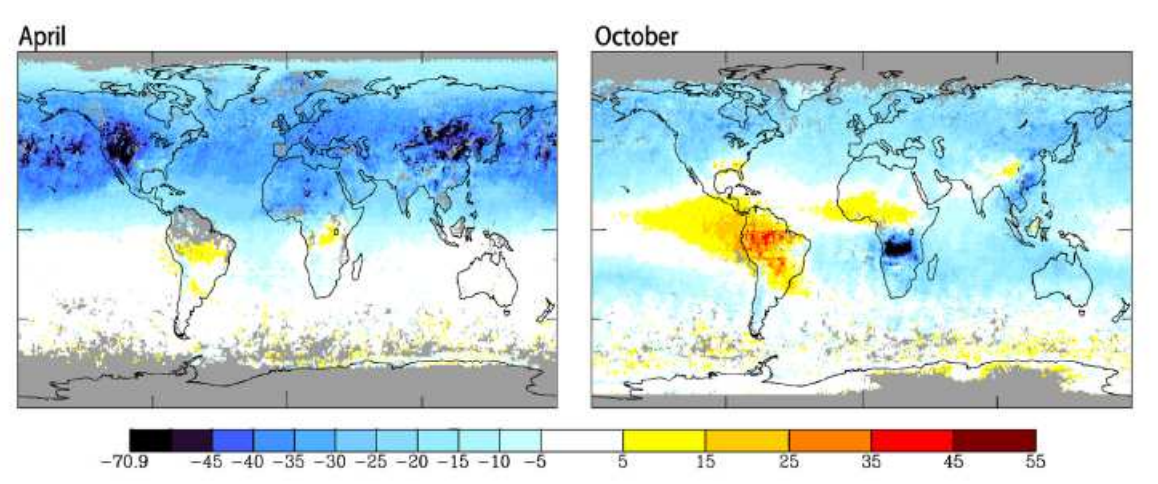
\includegraphics[width=\linewidth]{shindell2007plot}
\caption{Differences between the chemical transport multi-model mean CO and MOPITT V3 CO for 2000-2004 (ppbv) at 500 hPa. The background CO field is 200 ppbv. Plot from \cite{shindell2006}.}
\label{fig:shindell2007plot}
\end{figure*}
%
Another study, conducted by \cite{shindell2006} compared 26 different chemical transport models (CTMs) and found that they successfully reproduced the large scale spatial and temporal features of CO. However, the study also revealed significant biases between modeled and observed CO (See Figure \ref{fig:shindell2007plot}). Note that the average CO concentration is underestimated in the northern hemisphere during April and over the biomass burning regions of Africa during October. It turns out that CO concentrations are consistently underestimated in the northern hemisphere throughout the year \cite{shindell2006}. This is due to the underestimation of CO surface emissions caused by anthropogenic activity. Furthermore, the variability between the individual models was large even when the mean agreed with the observations. Again, this is due to incorrect estimations of emissions from NHMCs and gas oxidation. The study also found that transport was not as important as differences in NHMC estimates. \cite{liu2010} used the GEO-Chem CTM to analyze CO variation over tropical latitudes. The results were compared to the Microwave Limb Sounder (MLS) and Tropospheric Emission Satellite (TES) retrievals of CO. Again, spatial and seasonal CO variability was captured but there were underestimations in the biomass burning in the southern latitudes. The study also showed a temporal displacement in CO seasonal maxima in the troposphere over South America. The findings were linked to erroneous vertical transport and NHMC sources. Another study was conducted by \cite{ott2011}) concerning the influence of convective transport on CO fields. They perturbed the GEOS-5 convective parameters in an ensemble of eight simulations. The parameter changes caused large variability on CO concentrations over Africa, Indonesia, and South America. These areas notably feature significant biomass burning and convection in the lower atmosphere. The aforementioned results point to similar issues with modeling CO distribution: uncertainties in source estimates and in the transport. It is clear that one must better constrain estimates of CO sources to increase the accuracy of the CO simulations that rely on them.
\subsection{Estimation of CO Sources}
\label{sec:estimating co}
%

The two most common methods of calculating CO emissions are referred to as the bottom-up, and top-down approaches. The former method relies on regional and international energy statistics for estimates of both fossil fuel and biofuel sources. This data is combined with  geo-information such as population statistics, road type, and land cover data to approximate anthropogenic sources of CO. However, these data are often extrapolated in space and time. For example, statistics from countries with limited data are replaced with information from western countries \cite{streets2003}. For biomass burning, satellite observations are combined with ecosystem types to produce CO emission estimates. Despite this, it is still difficult to constrain burned area and fuel loads. \cite{van2010} showed that biomass burning calculations are uncertain to a minimum of 20$\%$.

The top-down approach uses ideas from the field of inverse modeling. This method attempts to minimize the differences between CTM simulations and observed CO concentrations by adjusting sources of CO. Most studies have used low-resolution Bayesian methods. That is, emissions are grouped by region and continent. Emissions are then scaled with respect to each unit to minimize the residual error between the model and the observations. However, this process leads to aggregation errors which have been shown to significantly impact emission estimates \cite{jiang2011}. Another top down approach considers techniques that fall under variational methods. Four dimensional variational data assimilation (4D-Var) is one such technique. 4D Var uses so called adjoint methods, which have the advantage of allowing emission estimates to be made at the native resolution of the CTM. These methods have immediate problems concerning data resolution limits in both the spatial and temporal domain. Aircraft and surface based observations don't guarantee a well constrained estimate on CO sources. \cite{jones2009} used CO retreivals from TES and MOPITT to constrain sources using the GEOS-Chem CTM. They found that differences in \textit{a posteriori} emission estimates were roughly 20$\%$ of the \textit{a priori} source information.

\section{Objective of Manuscript}
\label{sec:scope}

To summarize the previous sections, it is apparent that model biases are a challenge for the inverse modeling of CO emissions. Both satellite and surface CO data streams are insufficient to quantify emissions on regional subscales. Combining datasets is one solutions of overcoming the data sparsity problems. However, calculating covariances between the different streams of data can prove to be challenging. In this manuscript we use statistical methods to model CO fields. These methods avoid calculating model biases and covariances. This allows combinations of multivariate data to be included in the modeling of CO concentrations. It will also circumvent the challenges associated with model biases. This gain comes at the cost of losing information about the structure of the model. In particular, the free parameters of statistical models are often difficult to interpret outside of a handful of toy models. Our long term goal is to use a statitical approach to estimate CO sources. As a first step, the work presented in this report is focused on predicting CO concentrations using neural networks. If we can successfully predict CO fields then that information will lead to better estimates of CO sources.

First, the reader will be introduced to notion of artificial neural networks. The notion of training a neural network will be discussed, along with a derivation of the back-propagation algorithm. The network will applied to a nonlinear univariate regression problem. Then we attempt to model a Lorentz dynamical system using a neural network generator and discuss some limitations of FFNNs. Finally, we train the network on the GEOS-Chem chemical transport model to predict yearly CO fields.